\documentclass[10pt,a4paper]{article}
\usepackage[margin=2cm]{geometry}
\usepackage{amsmath,amssymb,booktabs,graphicx,caption,xcolor,float,hyperref,tikz}
\usetikzlibrary{arrows.meta,positioning,calc}
\hypersetup{colorlinks=true,linkcolor=blue!50!black,urlcolor=blue!50!black}
\captionsetup{font=small,labelfont=bf}
\title{\vspace{-1.2cm}\textbf{Steering a swarm that cannot prove anything}\\[2pt]
\large Simulation 1 (days and nights), setup \texttt{task003-nosolution}}
\author{LLM-free simulator; report of 17 October 2026; runs of 16 October 2026\\
\small Same structure as the gold-standard report on \texttt{task003-symmetric}; mirrors the Simulation 2 report of the same date.}
\date{}
\begin{document}
\maketitle
\vspace{-1cm}

\paragraph{How the simulator works.} The world, \texttt{task\_003}, has three candidate allocations; A0 is the
correct one. Each of 24 agents is given one true fact and reasons as an exact Bayesian: its \emph{belief} is the
exact probability of A0, A1 and A2 given the facts it currently remembers. An episode has 30 rounds, each a day
and a night. During the day the agents act one at a time in a new random order: an agent reads $q$ posts drawn at
random from a shared \emph{board} (never its own), adds their facts to its memory, recomputes its belief,
\emph{votes} by probability matching (a vote drawn from its belief) and posts one remembered fact that supports
its vote. At night a \emph{controller} with a target, A0 (truth) or A2 (false), reads $q_c$ agent posts and,
unless the \emph{vote gate} (at least 75\% of them from agents voting for its target) silences it, posts the $b$ facts from one shared pool that best support
its target. The board is then cleared, keeping only the controller's new posts. At each dawn every remembered fact is
forgotten with probability $1-\rho$ and comes back if read again. Every episode is run three times with the same
random draws: without a controller (\emph{silent}), with the controller targeting A0 and with the one targeting
A2.

\paragraph{The facts at the start.} All facts are true, and no set of them proves any allocation: the agents'
evidence is a coin flip between A0 and A2, and one pool serves both targets (Table~\ref{tab:facts}).

\begin{table}[H]
\centering\small
\caption{Facts available at the start and what each set implies, $P(\text{A0}, \text{A1}, \text{A2} \mid \text{facts})$.}
\label{tab:facts}
\begin{tabular}{lcc}
\toprule
set of facts & facts & $P(\text{A0}, \text{A1}, \text{A2})$ \\
\midrule
agents' facts, all together (24 agents, one fact each) & 15 distinct & (0.5, 0, 0.5): no proof \\
shared pool (both targets) & 12, all new to the agents & (0.37, 0.26, 0.37) \\
agents' facts + pool & 27 distinct & (0.75, 0, 0.25) \\
\bottomrule
\end{tabular}
\end{table}

\paragraph{The runs.} Posts read by an agent $q \in \{3, 6, 12\}$; posts read by the controller
$q_c \in \{3, 6, 12, 24\}$; facts posted per night $b \in \{1, \dots, 9\}$; memory $\rho \in \{1, 0.875, \dots,
0.125\}$ (8 values; this report shows $\rho = 1, 0.75, 0.5, 0.25$ like the gold standard, all 8 are in the notebook
\texttt{shared\_analysis/gold\_standard/explorer.ipynb}); vote gate on and off; 1{,}000 episodes per setting
(3{,}480 settings). Unless stated otherwise: $q = 6$, $q_c = 12$, $b = 1$, gate on. Cells shared with the
7 October run reproduce it exactly.

\paragraph{Summary.} The 24 agents' evidence is a coin flip between A0 (the truth) and A2, and no set of facts can
prove either. \textbf{Without a proof to defend, every swarm is steerable}: either controller tips it within a few
days at every memory, full memory included (Figure~\ref{fig:votes}). \textbf{The budget, not memory, is the main
axis}: one fact per night steers best and is twenty to a hundred times more effective per fact than nine, while large
budgets backfire and lower the false controller's own target share, most with full memory
(Figures~\ref{fig:timeseries}, \ref{fig:perfact}, \ref{fig:strength}). Susceptibility, readability and efficiency fall
together at large budgets, and reading more posts helps the controller when agents forget and hurts it with full memory
(Figures~\ref{fig:phaserq}--\ref{fig:phaseqx}).

\section{Quantities}\label{sec:quantities}

\paragraph{Votes.} With $n_{a,t}$ the number of agents whose vote on day $t$ is answer $a$ and $N_t = 24$ (every
agent votes every day; before the first day nobody has voted and we set $x_{a,0} = 0$),
\begin{equation}\label{eq:share}
x_{a,t} = n_{a,t}/N_t .
\end{equation}

\paragraph{Paired susceptibility.} Following \texttt{BLACKBOARD\_OBSERVABLES\_AND\_EFFICIENCIES} (\S3), for a
controller policy $\pi$ and an answer $a$,
\begin{equation}\label{eq:chi}
\chi^{(a)}_{\pi,t} \equiv G^{(a)}_t(\pi) = \mathbb E\bigl[x^{\pi}_{a,t} - x^{\rm base}_{a,t}\bigr],
\end{equation}
the mean over episodes of the difference between the controlled run and the silent run of the same episode. We
report it on the controller's own target: $G_t \equiv G^{(0)}_t(\pi^{+})$ for the controller targeting A0 and
$G_t \equiv G^{(2)}_t(\pi^{-})$ for the one targeting A2.

\paragraph{Target and state.} The target $Z \in \{\text{A0}, \text{A2}\}$ is drawn by a fair coin. The state $X$
on day $t$ is the vote of a randomly chosen agent, $X \in \{\text{A0},\text{A1},\text{A2}\}$. Each episode $e$ of arm $s$
(silent 0, target A0 $+$, target A2 $-$) contributes its vote shares $y^{(e)}_s(x) = x_{x,t}$, and
\begin{equation}\label{eq:P}
P_s(x) = \frac1E\sum_{e=1}^{E} y^{(e)}_s(x), \qquad E = 1000 .
\end{equation}

\paragraph{Readability and efficiency.} With $Q = \frac12(P_+ + P_-)$ and $\mathrm{KL}(p\Vert q) = \sum_x p(x)\log_2[p(x)/q(x)]$,
\begin{equation}\label{eq:I}
I(Z;X) = \tfrac12\,\mathrm{KL}(P_+\Vert Q) + \tfrac12\,\mathrm{KL}(P_-\Vert Q),
\end{equation}
the information the state carries about the target (at most 1 bit). The controllers' total change from silence
splits exactly into a directed and an undirected part,
\begin{equation}\label{eq:C}
C = \tfrac12\,\mathrm{KL}(P_+\Vert P_0) + \tfrac12\,\mathrm{KL}(P_-\Vert P_0) = I(Z;X) + \mathrm{KL}(Q\Vert P_0),
\end{equation}
and the efficiency is the directed share,
\begin{equation}\label{eq:eta}
\eta = I(Z;X)/C .
\end{equation}
Silence sometimes never shows a value of $X$ that a controller reaches, which would make $C$ infinite. Before
computing any KL, every arm's distribution therefore receives the same pseudo-count of $\alpha = 0.5$ episodes per
value of $X$ ($K$ values),
\begin{equation}\label{eq:smooth}
\tilde P_s(x) = \frac{E\,P_s(x) + \alpha}{E + \alpha K}.
\end{equation}
With $\alpha = 1$ instead, $\eta$ changes by at most 0.004; without it, by at most 0.005 where $C$ is finite. $\eta$ is not defined when $C < 0.01$ bits (no measurable change);
such values are left blank. Equation~(\ref{eq:C}) holds in the data to $4\times10^{-15}$ bits.

\paragraph{Cost.} $F_t$ is the number of facts the controller has posted on the nights before day $t$ (mean per
episode); the gain per fact is $G_t/F_t$, and the marginal susceptibility is the slope between neighbouring
budgets,
\begin{equation}\label{eq:slope}
\frac{\Delta G}{\Delta b} = \frac{G(b^{(k+1)}) - G(b^{(k)})}{b^{(k+1)} - b^{(k)}} .
\end{equation}
Episode $e$ uses the same random draws at every budget, so the slope is estimated from per-episode differences,
$[x^{(e)}_{\text{target},t}(b^{(k+1)}) - x^{(e)}_{\text{target},t}(b^{(k)})]/(b^{(k+1)} - b^{(k)})$, whose mean is
Eq.~(\ref{eq:slope}) and whose standard error gives the 95\% intervals (typically $\pm0.006$--$0.02$, about 30\%
narrower than for two independent means).

\section{Votes over time}

\begin{figure}[H]
\centering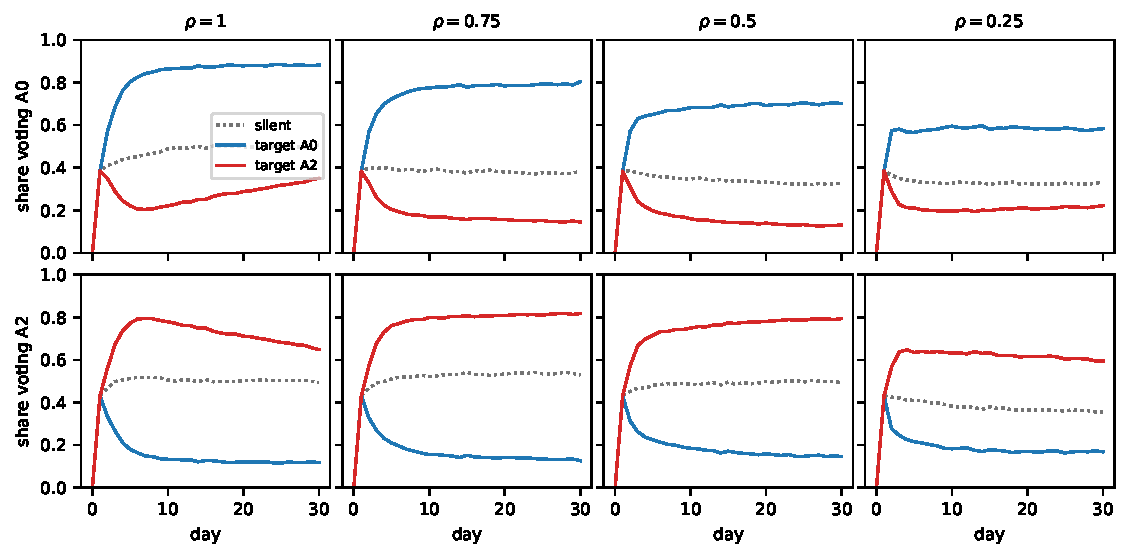
\includegraphics[width=0.95\linewidth]{figures/fig_votes.pdf}
\caption{Share of agents voting A0 (top) and A2 (bottom) at the end of each day, Eq.~(\ref{eq:share}), without a
controller (dotted), with the controller targeting A0 (blue) and A2 (red); one column per memory $\rho$. $q = 6$,
$q_c = 12$, $b = 1$, gate on. Day 0: nobody has voted yet, every share is 0.}
\label{fig:votes}
\end{figure}

\begin{itemize}\itemsep1pt
\item \textbf{Without a controller the swarm stays split at every memory}: on day 30, 33--51\% vote A0 and 35--53\% A2;
  with heavy forgetting ($\rho = 0.25$) a third of the votes go to A1.
\item \textbf{Either controller tips it within a few days, at every $\rho$}: the truth controller raises A0 to 0.88,
  0.80, 0.70, 0.58 and the false controller A2 to 0.65, 0.82, 0.79, 0.59 for $\rho = 1, 0.75, 0.5, 0.25$.
\item \textbf{Unlike in \texttt{task003-symmetric}, full memory does not protect the swarm}: there is no proof to
  rebuild. Only the false controller's lead erodes with full memory (A2 at 0.79 on day 7, 0.65 on day 30).
\end{itemize}

\section{Observables as time series}\label{sec:time}

\begin{figure}[H]
\centering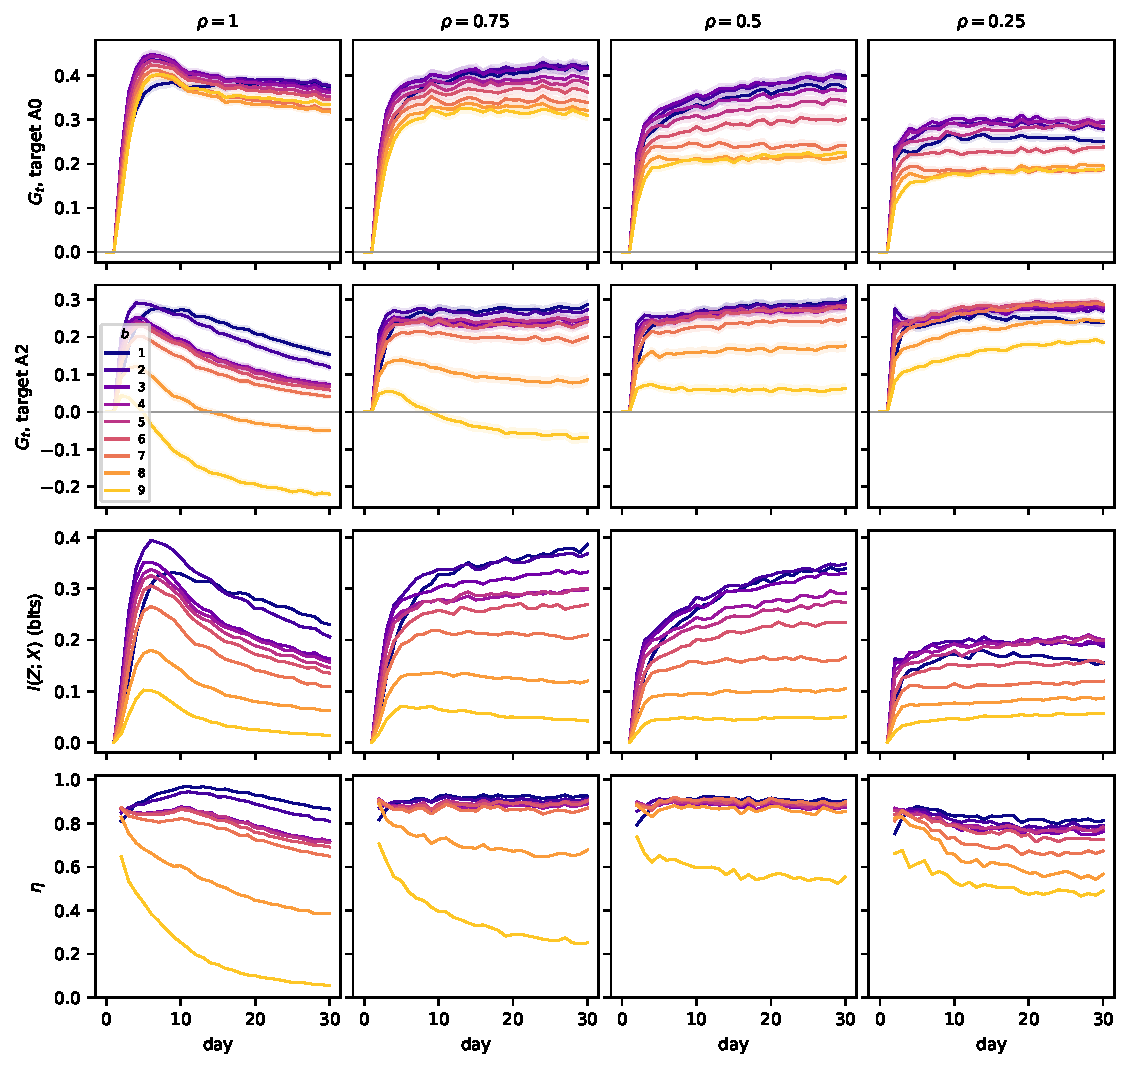
\includegraphics[width=0.95\linewidth]{figures/fig_timeseries.pdf}
\caption{All observables over the days, one column per memory $\rho$, one curve per budget $b$; $q = 6$,
$q_c = 12$, gate on. Rows: paired susceptibility $G_t$, Eq.~(\ref{eq:chi}), for target A0 and target A2 (bands:
95\% intervals; $G_0 = 0$); readability $I(Z;X)$, Eq.~(\ref{eq:I}); efficiency $\eta$, Eq.~(\ref{eq:eta}) (blank:
undefined).}
\label{fig:timeseries}
\end{figure}

\begin{figure}[H]
\centering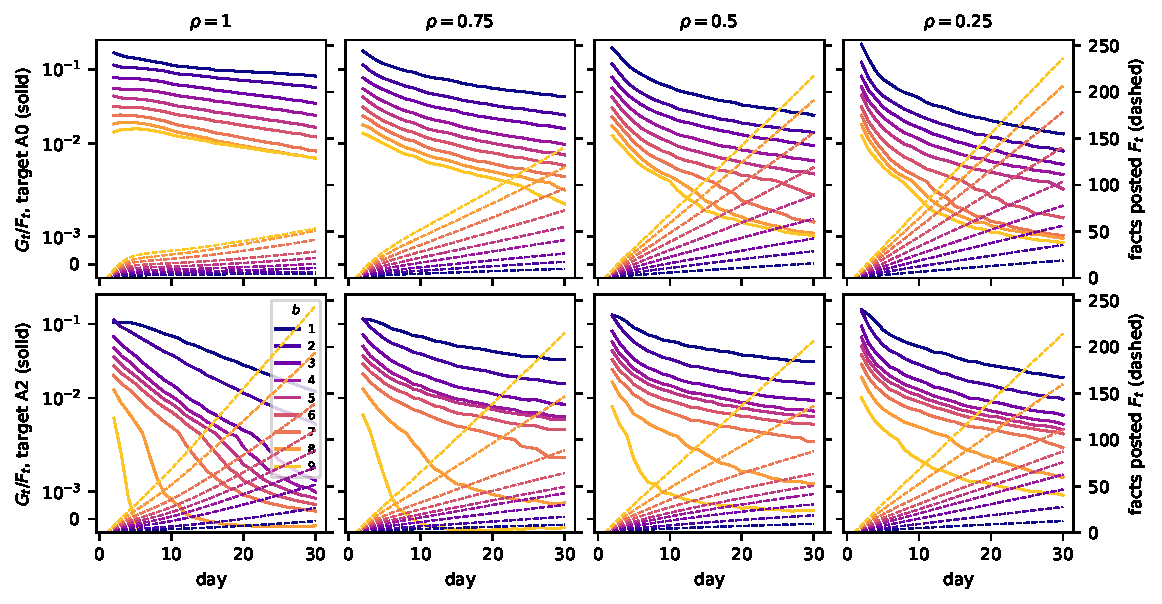
\includegraphics[width=0.95\linewidth]{figures/fig_per_fact.pdf}
\caption{Gain per fact $G_t/F_t$ (solid, left axis, log scale; shown once at least half a fact has been posted)
and facts posted $F_t$ (dashed, right axis), target A0 (top) and A2 (bottom), one colour per budget; $q = 6$,
$q_c = 12$, gate on.}
\label{fig:perfact}
\end{figure}

\paragraph{Susceptibility (Figure~\ref{fig:timeseries}, rows 1--2).}
\begin{itemize}\itemsep1pt
\item \textbf{Small budgets steer best}: on day 30, target A0, $G = 0.33$--$0.38$, $0.31$--$0.42$, $0.22$--$0.40$,
  $0.19$--$0.30$ for $\rho = 1, 0.75, 0.5, 0.25$, highest at $b \le 3$; target A2, $-0.22$ to $0.15$, $-0.07$ to $0.29$,
  $0.06$ to $0.30$, $0.19$ to $0.29$, highest at $b = 1$--2.
\item \textbf{Large budgets backfire}: at $b = 9$ the false controller \emph{lowers} the A2 share at $\rho \ge 0.75$
  ($-0.07$, $-0.22$), and the effect builds over the days. Likely reason, not tested directly: a large batch must
  include pool facts that also support A0, which agents keep.
\item \textbf{With full memory the false controller's gain decays} for every budget, as agents accumulate evidence
  for A0.
\end{itemize}

\paragraph{Readability and efficiency (rows 3--4).}
\begin{itemize}\itemsep1pt
\item \textbf{Readability falls with the budget}: on day 30, $I = 0.01$--$0.23$, $0.04$--$0.39$, $0.05$--$0.35$, $0.06$--$0.20$
  bits for $\rho = 1, 0.75, 0.5, 0.25$, highest at $b = 1$.
\item \textbf{Efficiency falls with the budget too}, from $0.81$--$0.93$ at small $b$ to $0.06$--$0.55$ at $b = 9$: large
  budgets push both controllers' swarms the same way (a common push), which $\eta$ counts as undirected.
\end{itemize}

\paragraph{Gain per fact and facts posted (Figure~\ref{fig:perfact}).}
\begin{itemize}\itemsep1pt
\item \textbf{One fact per night is far the most effective per fact}: on day 30, target A2, $\rho = 0.5$: $0.031$ per
  fact at $b = 1$ (10 facts) against $0.0003$ at $b = 9$ (207 facts); target A0, $\rho = 0.75$: $0.043$ against $0.002$.
\item \textbf{The false controller posts about 210 facts by day 30 at $b = 9$, at every memory}; the truth
  controller is silenced by the gate more often when agents remember (53 facts at $\rho = 1$, 141 at $\rho = 0.75$,
  217 at $\rho = 0.5$), because its target is the one the swarm already leans to.
\end{itemize}

\section{Phase diagrams}\label{sec:phase}

All panels on day 30, gate on; the susceptibility is for target A2 (grey number: its 95\% interval includes 0);
readability and efficiency are for the pair of targets.

\begin{figure}[H]
\centering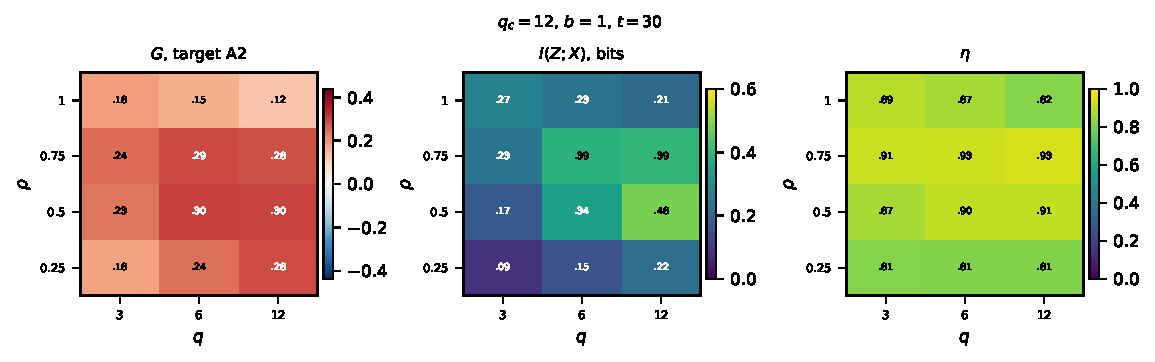
\includegraphics[width=0.98\linewidth]{figures/fig_phase_rho_q.pdf}
\caption{Susceptibility, readability and efficiency over memory $\rho$ and the posts each agent reads $q$;
$q_c = 12$, $b = 1$.}
\label{fig:phaserq}
\end{figure}

\begin{itemize}\itemsep1pt
\item \textbf{Reading more helps the controller except with full memory}: at $\rho = 0.25$, $G$ rises from $0.18$
  ($q = 3$) to $0.28$ ($q = 12$) and $I$ from $0.09$ to $0.22$ bits; at $\rho = 1$, $G$ falls from $0.18$ to $0.12$ and
  $I$ from $0.27$ to $0.21$.
\item \textbf{$\eta$ stays at 0.73--0.93} at $b = 1$.
\end{itemize}

\begin{figure}[H]
\centering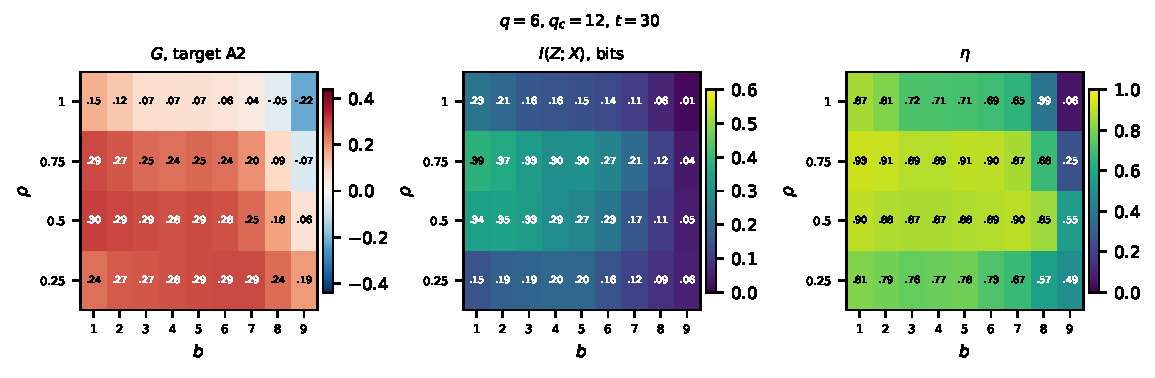
\includegraphics[width=0.98\linewidth]{figures/fig_phase_rho_x.pdf}
\caption{Susceptibility, readability and efficiency over memory $\rho$ and the budget $b$; $q = 6$, $q_c = 12$.}
\label{fig:phaserx}
\end{figure}

\begin{itemize}\itemsep1pt
\item \textbf{The budget is the main axis}: along every row $G$ falls at large $b$, most with full memory ($0.15$ at
  $b = 1$ to $-0.22$ at $b = 9$) and least with heavy forgetting ($0.24$--$0.29$, then $0.19$).
\item \textbf{$I$ and $\eta$ fall with $b$ in the same way}: $\eta$ from $0.75$--$0.93$ at $b = 1$ to $0.06$ ($\rho = 1$,
  $b = 9$).
\end{itemize}

\begin{figure}[H]
\centering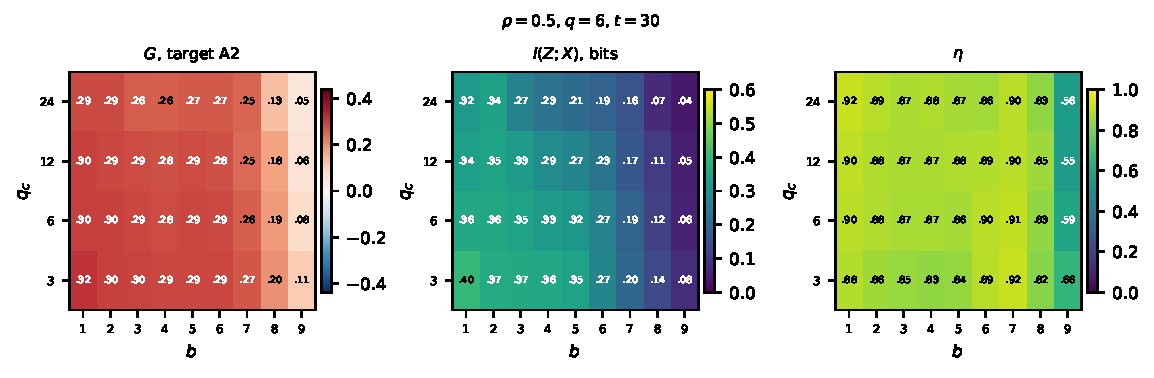
\includegraphics[width=0.98\linewidth]{figures/fig_phase_qc_x.pdf}
\caption{Susceptibility, readability and efficiency over the posts the controller reads $q_c$ and the budget $b$;
$\rho = 0.5$, $q = 6$.}
\label{fig:phaseqx}
\end{figure}

\begin{itemize}\itemsep1pt
\item \textbf{At $\rho = 0.5$ the budget dominates}: $G = 0.05$--$0.32$, $I = 0.04$--$0.40$ bits and $\eta = 0.55$--$0.92$,
  all falling at large $b$; the controller's reading changes $G$ by at most $0.03$ on average (mean $0.26$, $0.25$,
  $0.25$, $0.23$ for $q_c = 3, 6, 12, 24$).
\end{itemize}

\section{Susceptibility against the budget, and its slope}\label{sec:strength}

\begin{figure}[H]
\centering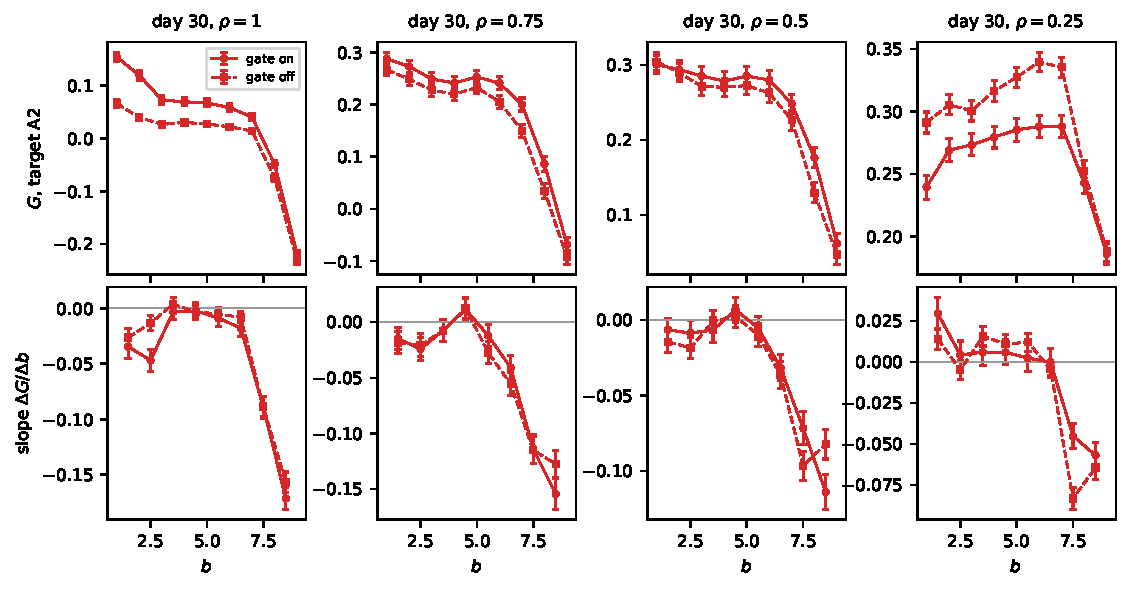
\includegraphics[width=0.95\linewidth]{figures/fig_gain_strength.pdf}
\caption{Top: $G$ on day 30, target A2, against the budget $b$, one panel per $\rho$; gate on (solid) and off
(dashed); bars: 95\% intervals. Bottom: the slope between neighbouring budgets, Eq.~(\ref{eq:slope}), with paired 95\%
intervals.}
\label{fig:strength}
\end{figure}

\begin{figure}[H]
\centering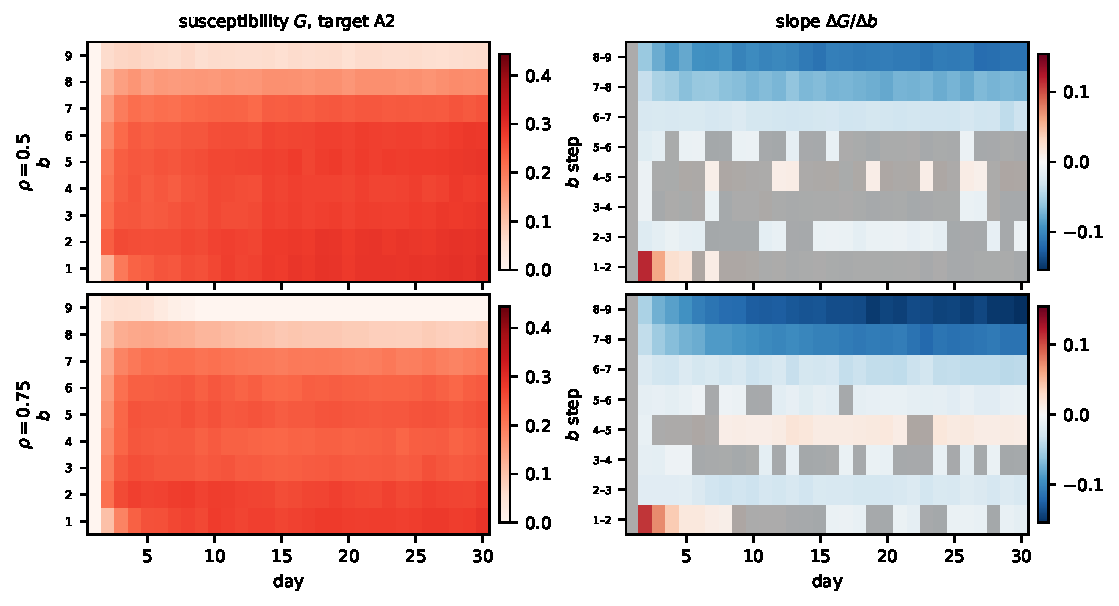
\includegraphics[width=0.95\linewidth]{figures/fig_strength_time.pdf}
\caption{$G$, target A2 (left), and its slope between neighbouring budgets (right) over the days ($x$) and the
budget ($y$), for $\rho = 0.5$ (top) and $0.75$ (bottom); $q = 6$, $q_c = 12$, gate on. Each row of the right panels
is one step between neighbouring budgets; faded cells: its paired 95\% interval includes 0.}
\label{fig:strengthtime}
\end{figure}

\begin{itemize}\itemsep1pt
\item \textbf{More budget rarely helps}: on day 30 the slope is significantly positive only for $b = 1 \to 2$ at
  $\rho = 0.25$ ($+0.03$); everywhere else it is zero or negative.
\item \textbf{The last steps are strongly negative}: $b = 8 \to 9$ costs $-0.17$ ($\rho = 1$), $-0.15$ ($\rho = 0.75$),
  $-0.11$ ($\rho = 0.5$), $-0.06$ ($\rho = 0.25$) per extra fact per night.
\item \textbf{The backfire builds over the days} (Figure~\ref{fig:strengthtime}): the negative slopes at large $b$ grow
  from day 5 to day 30, while the first step's positive slope fades.
\item \textbf{Turning the gate off lowers $G$ when agents remember} ($-0.01$ to $-0.09$ at $\rho = 1$) and raises it
  slightly with heavy forgetting (up to $+0.05$ at $\rho = 0.25$).
\end{itemize}

\paragraph{No proofs here.} In \texttt{task003-nosolution} no set of facts proves any allocation, so the
gold standard's ``who holds the proof'' section has no counterpart.

\section{Conclusions}

\begin{enumerate}\itemsep2pt
\item \textbf{Without a proof to defend, every swarm is steerable.} Either controller tips it at every memory,
  including full memory.
\item \textbf{The budget, not memory, is the main axis.} One fact per night steers best; large budgets backfire,
  most with full memory, because the shared pool runs out of facts on the target's side.
\item \textbf{Susceptibility, readability and efficiency all fall at large budgets}; $\eta$ drops as both controllers
  push the swarm the same way.
\item \textbf{Reading more posts helps the controller when agents forget and hurts it with full memory.}
\item \textbf{Compared with Simulation 2}: the same picture at small strengths. Simulation 2's controller has
  30 messages in total, so it cannot flood the board; there the false controller's gain does not turn negative, but
  with full memory a faster rate still gains less (the rate reversal).
\end{enumerate}

\paragraph{Caveats.} One world, 24 exact-Bayesian agents voting by probability matching, one controller policy
posting a fixed batch each night; 1{,}000 episodes per setting (95\% intervals on $G$ about $\pm0.02$). Information
is plug-in from 1{,}000 episodes per arm. Data: \texttt{results/simulation\_1/2026-10-16\_sim1\_pm\_nosolution\_fine};
tables: \texttt{results/gold\_standard/2026-10-16/}; code: \texttt{analysis/task003\_llm\_free/shared\_analysis/gold\_standard/}.

\end{document}
